\documentclass[10pt,letterpaper]{article}
\usepackage[dvipsnames]{xcolor}

\usepackage{outlines}
\usepackage{amsmath}
\usepackage{tikz}
\usepackage{hyperref}
\usepackage{enumitem}
\usepackage{caption}
\usepackage{subcaption}
\DeclareCaptionOptionNoValue{centering}{\centering} % Make sure everything is centered in subs
\captionsetup[sub]{centering}

\usepackage{multirow}
\usepackage{cancel}
\usepackage{float}

\usepackage{parskip}

\usepackage{slantsc,lmodern}

\usepackage{pgfplotstable,booktabs}
\usepackage{textcomp}
\usepackage{gensymb}

\usepackage{paralist}

\usepackage{amsmath}
\usepackage{tikz}
\usepackage{hyperref}

\usepackage{pst-node}
\usepackage{auto-pst-pdf}

\usepackage[paper=a4paper,margin=1.25in]{geometry}

\makeatletter
\g@addto@macro\@floatboxreset\centering
\makeatother

\newcommand{\volume}{{\ooalign{\hfil$V$\hfil\cr\kern0.08em--\hfil\cr}}}

\author{Thaddeus Hughes \\ hughes.thad@gmail.com \\ thaddeus-maximus.github.io}
\date{\today}
\title{Documentation and Validation of EveryCalc's General Mechanism Tool}

\begin{document}
	\maketitle
	
	\begin{abstract}
		Once upon a time, the man, myth, and legend built the \href{https://johnvneun.com/calc}{\underline{JVN Calc}}. Since then many people have been devising tweaks and improvements to the system to handle more specific use cases and add additional analysis features. One of the more interesting features is \textit{transient analysis}, also known as \textit{time-to-target} or \textit{sprint-distance} analysis. This considers not only the loads and motors acting on the system, but the accelerated mass, and allows for much more complex analysis of variable loads as well.
	\end{abstract}

	\section{DC Motor Behavior}
	To begin with, we're going to consider DC motor behavior.

	\begin{figure}[H] \centering
	\begin{tikzpicture}[x=4.0in,y=2.0in]
	  %\fill[lightgray] (1.0,0)--(0,1.0)--(0,0)--cycle;
	  \draw[black] (-0.1,0)--(1.1,0) node[pos=0.3,below]{\bf Speed $\omega$, RPM};
	  \draw[black] (0,-0.1)--(0,1.1) node[pos=0.9,above,rotate=90,teal]{\bf $T$, N-m}
	  node[pos=0.65,above,rotate=90,RawSienna]{\bf $I$, A};
	  \draw[black] (1,-0.1)--(1,1.1) node[pos=0.24,below,rotate=90,red]{\bf $P$, W}
	  node[pos=0.61,below,rotate=90,blue]{\bf Efficiency $\eta$, \%};

	  \draw[teal, ultra thick] (1.0,0)--(0,1.0);
	  \draw[RawSienna, ultra thick] (1.0,0.1)--(0,0.8);
	  \draw[red, ultra thick] (0,0) parabola bend (0.5,1.0) (1.0,0.0) ;
	  \draw[blue, ultra thick] (0,0)--(0.8,0.99) parabola bend (0.82,1.0) (1.0,0.0) ;
	  
	%  \draw[gray, dashed] (0.82,0) -- (0.82, 1) node[pos=0,below, black]{\bf 70-85\% $\omega_{free}$};
	  
	%  \draw[gray, dashed] (1,1) -- (0.82, 1) node[pos=0,right, black]{\bf $\eta_{peak}$};
	\end{tikzpicture}
	\caption{Complete motor curve.}
	\end{figure}

	The current and torque, which we are most interested in, could be expressed mathematically as
	\begin{align} \label{eq:motor_torque_curve}
		T_m(\omega_m) &= T_{m,stall} \frac{\omega_m-\omega_{m,free}}{\omega_{m,free}} \\
		I_m(T_m) &= (I_{m,stall} - I_{m,free}) \frac{T_m}{T_{m,stall}} + I_{m,free}
	\end{align}

	\section{Gearbox and Coupled Mechanism}

	Multiple, $N$ motors could be connected to a gear ratio $G$.

	\begin{align}
		T_{g}(\omega_{g}) &= N \ G \ T_m(G \omega_{g}) \\
		I_{g}(\omega_{g}) &= N I_m(T_{g} / G)
	\end{align}

	The torque might be limited by a clutch, or by some other friction interface (such as carpet against a wheel). The gearbox also may have non-perfect efficiency, so an efficiency factor can be applied here.

	\begin{align}
		T_{g}(\omega_{g}) = min \left\{
	        \begin{array}{ll}
	        	N \ G \ T_m(G \omega_{g}) \eta_{g} \\
	            N \mu r
	        \end{array}
	    \right. ,
	\end{align}

	where $N$ is the normal force, $\mu$ is the friction coefficient, and $r$ is the radius of the friction interface.

	Let's consider the following generalized mechanism. Gearbox torque is applied, as is a resistance $M_resist$. This could be computed from gravity, spring force... or something else entirely.

	\begin{figure}[H] \centering
	\begin{tikzpicture}[x=1.0in,y=1.0in]
		\draw[ultra thick] (0,0) circle (0.1);
		\fill[black] (0,0.1)--(0,0)--(0.1,0) arc[start angle=0, end angle=90, radius=0.1]--cycle;
		\fill[black] (0,-0.1)--(0,0)--(-0.1,0) arc[start angle=180, end angle=270, radius=0.1]--cycle;
		\draw[ultra thick, black] (0,0) circle (0.5);
		
		\draw[ultra thick, red, ->] (-0.1,0.6) arc[start angle=99.6, end angle=180, radius=0.608] node[pos=0.7,left]{$M_{resist}$};
		\draw[ultra thick, OliveGreen, ->] (0.1,0.6) arc[start angle=80.4, end angle=0, radius=0.608] node[pos=0.7,right]{$T_{g}$};
		
		\draw[ultra thick, blue, ->] (0,0.2) arc[start angle=90, end angle=-30, radius=0.2] node[pos=0.0,above]{$I_{sys} \alpha_{g}$};
	\end{tikzpicture}	
	\caption{Free-body diagram for the flywheel, with additional resistance $M_{resist}$.}
	\end{figure}

	Using conservation of angular momentum,
	\begin{align}
		%\sum M &= I \alpha + \cancelto{0 \ \mbox{(no mass transfer)}}{\sum \dot{m}(...)}  \\
		T_{gbx} - M_{resist} &= I_{sys} \alpha_{g} \\
		\alpha_{g} &= \frac{d}{dt} \omega_{g}
	\end{align}

	Solving yields the state equations

	\begin{align}
		\frac{d}{dt} \omega_{g} &= \frac{T_{g}(\omega_{g}) - M_{resist}}{I_{sys}} \\
		\frac{d}{dt} \theta_{g} &= \omega_{g}
	\end{align}

	With initial conditions

	\begin{align}
		\omega_g(t=0) = \theta_g(t=0) = 0 
	\end{align}

	This could be adapted to the case of a linear mechanism by
	\begin{align}
		M_{resist} = r F_{resist} \\
		\omega_g   = v / r \\
		\theta_g   = x / r \\
		I_{sys}    = m r^2
	\end{align}

	\section{Current Limit}

	\begin{align}
		V_{motor} = V_{battery} - I_{motor}(\omega_m, \frac{V_{motor}}{V_{motor,nominal}}) R \\
		V_{motor} = V_{battery} - [(I_{stall} - I_{free})\frac{\omega_{m} - \omega_{free}}{\omega_{free}} + I_{free}] \frac{V_{motor}}{V_{motor,nominal}} R \\
		V_{motor} = \frac{V_{battery} + R (I_{stall}-I_{free}) \frac{\omega_m}{\omega_{free}}}{1 + \frac{R}{V_{motor,nominal}} I_{stall}}
	\end{align}

	\section{Steady-State Calculations}
	A fair bit of information can be gained from steady-state analysis, so EveryCalc produces these numbers as well. The first is the free speed, given as

	\begin{align}
		v_{free} = \frac{\omega_{m,free} r}{G}
	\end{align}

	JVN's speed loss constant ($SLC$) is used to compute the JVN adjusted speed

	\begin{align}
		v_{JVN} = SLC \times v_{free}
	\end{align}

	The running speed can be found at the steady-state condition of $T_g = M_{resist}$. Currently, $M_{resist}$ is evaluated at all parameters being zero, though the use of a numerical method such as bisection could be used to make this a more interesting number.

	\section{Validation}
	Validation and verification are important aspects in trusting a tools' accuracy. This can be done either to test results or prior art. I would love to obtain test data for sprint distances (and it would be simple to obtain) but currently no such data exists. As such I will compare my results to a couple pre-existing tools.

	\newpage
	\subsection*{Case A: Drivetrain}
	We can compare a drivetrain to the \href{https://www.chiefdelphi.com/t/paper-jvns-mechanical-design-calculator-2016/146281}{\underline{JVN calculator}}.

	\begin{figure}[H]
		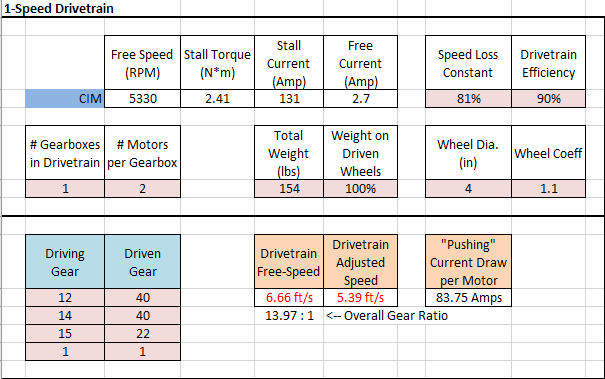
\includegraphics[width=0.80\textwidth]{validation/mechanism_JVN_A.png}
	\end{figure}

	\begin{figure}[H]
		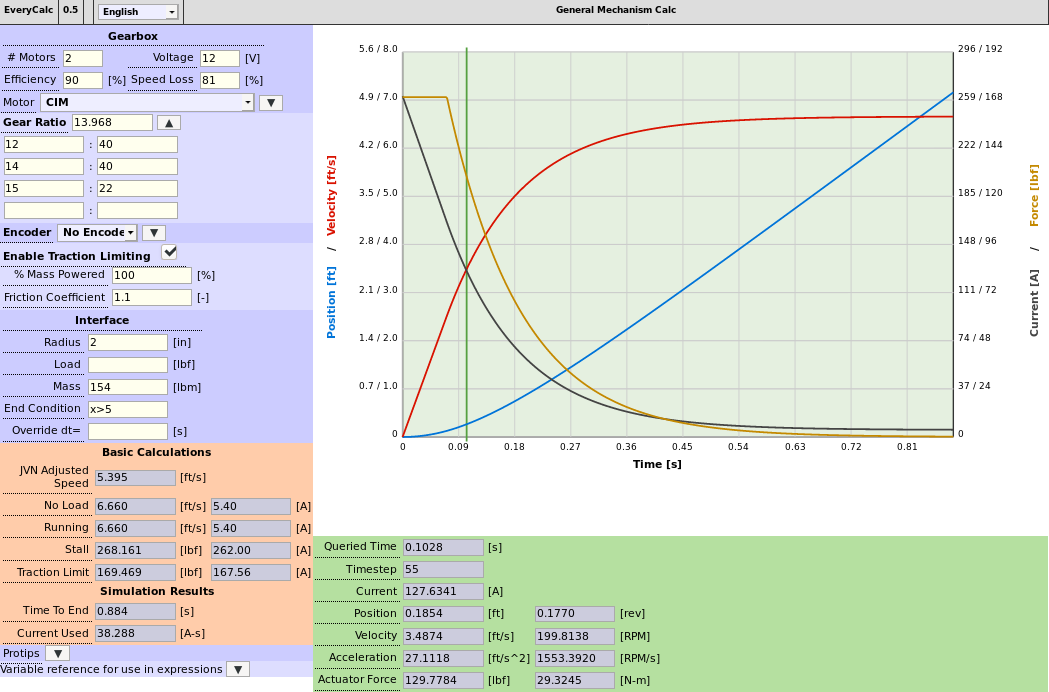
\includegraphics[width=0.95\textwidth]{validation/mechanism_EC_A.png}
	\end{figure}

	\begin{table}[H]
	\begin{tabular}{llll}
	                & JVN & EveryCalc V0.5 & \\ \cline{1-4} 
	Free Speed      & 6.66 & 6.669 & $ft \ / \ s$ \\
	Adjusted Speed  & 5.39 & 5.395 & $ft \ / \ s$ \\
	Current at Traction Limit & $83.75 \times 2 =$ 167.5 & 167.56 & $A$
	\end{tabular}
	\end{table}

	No issues here other than minor rounding errors.

	\newpage
	\subsection*{Case B: Mechanism}
	We can compare a drivetrain to the \href{https://www.chiefdelphi.com/t/paper-jvns-mechanical-design-calculator-2016/146281}{\underline{JVN calculator}}.

	\begin{figure}[H]
		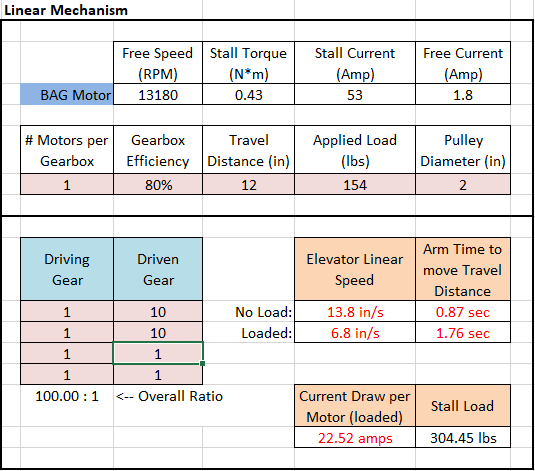
\includegraphics[width=0.52\textwidth]{validation/mechanism_JVN_B.png}
	\end{figure}

	\begin{figure}[H]
		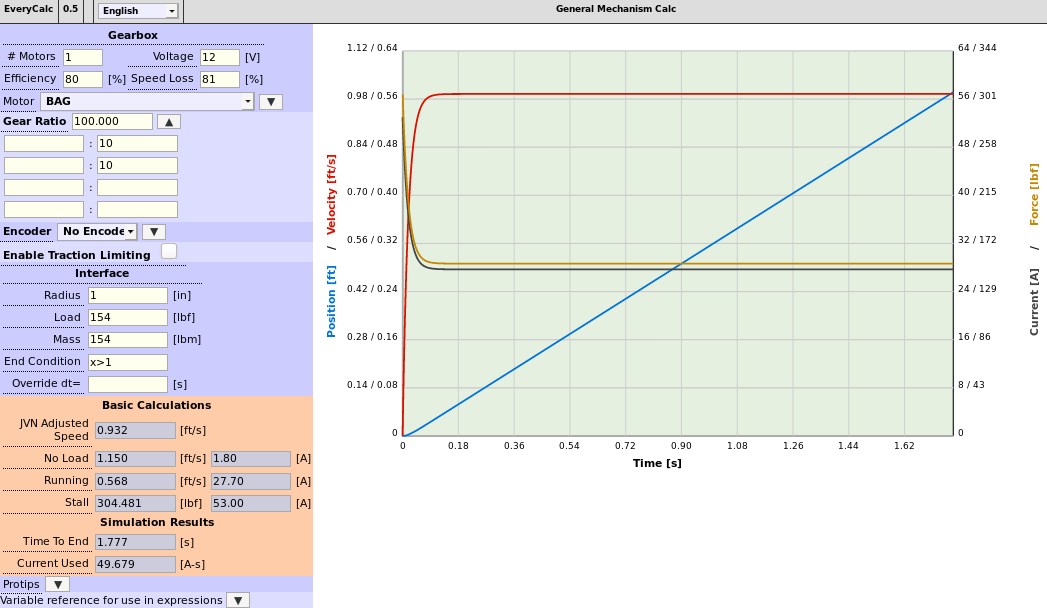
\includegraphics[width=0.95\textwidth]{validation/mechanism_EC_B.png}
	\end{figure}

	\begin{table}[H]
	\begin{tabular}{llll}
	                & JVN & EveryCalc V0.5 & \\ \cline{1-4} 
	Free Speed      & 1.150 & 1.150 & $ft \ / \ s$ \\
	Loaded Speed    & 0.566 & 0.568 & $ft \ / \ s$ \\
	Loaded Current  & 22.52 & 27.70 & $A$ \\
	Stall Force     & 304.5 & 304.481 & $lbf$ \\
	Time to Target  & 1.76  & 1.777 & $s$
	\end{tabular}
	\end{table}

	There is a discrepancy in the loaded current number. I believe this is an error in JVN's calculator- his calculation of current does not take into consideration the gearbox efficiency, so is optimistic on current draw.

	Note that EveryCalc predicts this mechanism taking slightly longer than JVN does- this is because of the time required to accelerate this mechanism, which the JVN calc does not consider.

	\newpage
	\subsection*{Case C: Time-To-Target}
	We can compare a drivetrain to a \href{https://www.chiefdelphi.com/t/paper-jvn-calc-apalrds-time-to-distance/146546}{\underline{modified JVN calculator by apalrd}}.

	\begin{figure}[H]
		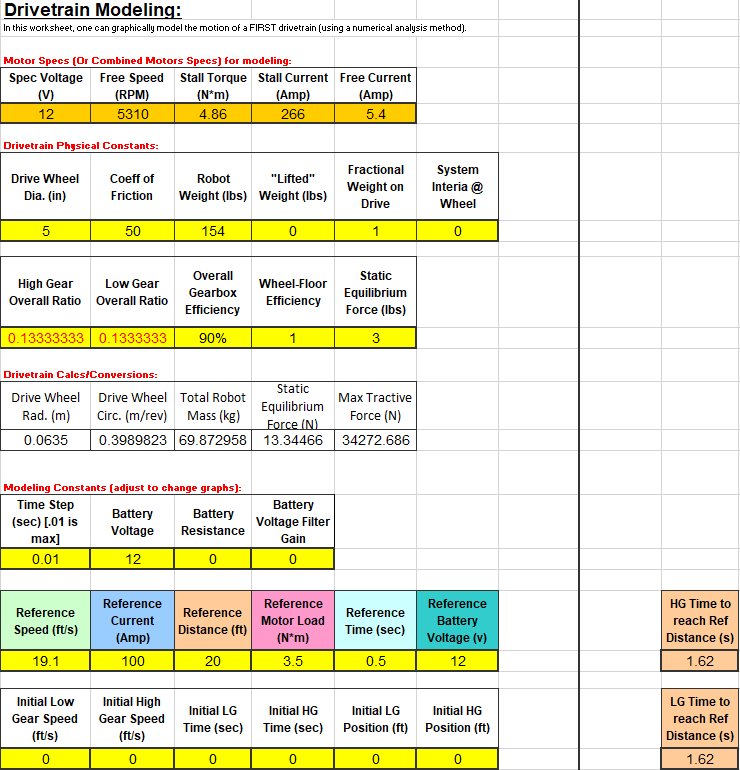
\includegraphics[width=0.75\textwidth]{validation/mechanism_JVN_apalrd_C.png}
	\end{figure}

	\begin{figure}[H]
		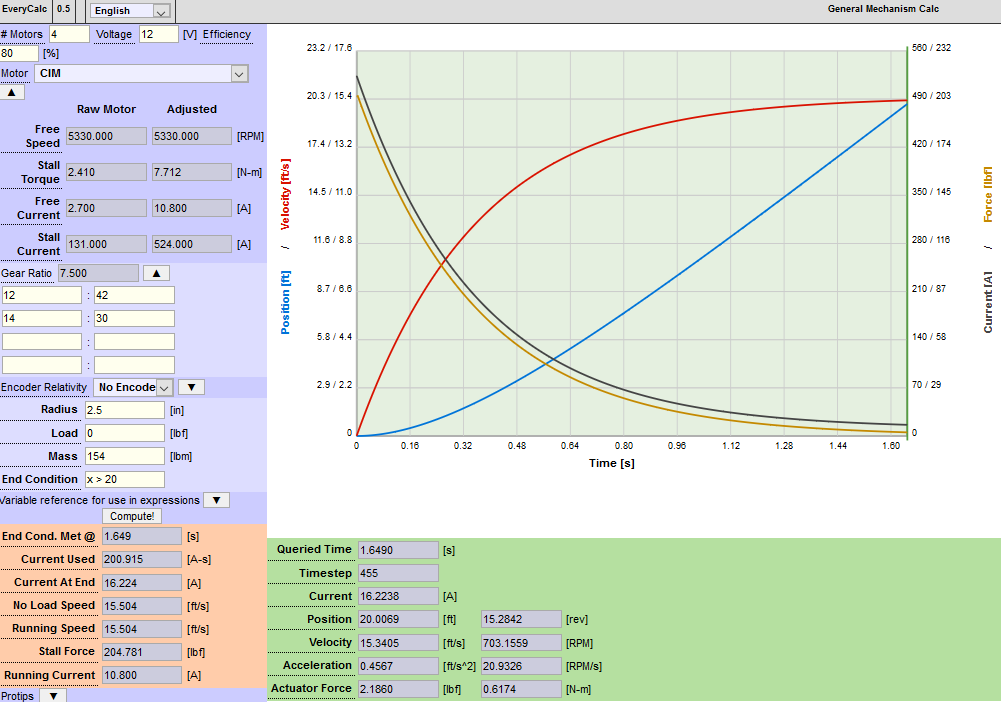
\includegraphics[width=0.95\textwidth]{validation/mechanism_EC_C.png}
	\end{figure}

	\begin{table}[H]
	\begin{tabular}{llll}
	                & JVN/apalrd & EveryCalc V0.5 & \\ \cline{1-4} 
	Time to Target  & 1.62  & 1.611 & $s$
	\end{tabular}
	\end{table}

	Effectively the same result. Note: the modified calculator with sprint distance does not consider wheel slip due to friction, hence traction limiting is disabled in everycalc for a fair comparison.

\end{document}